\documentclass[11pt]{report}
\usepackage[utf8]{inputenc}
\usepackage[dutch]{babel} %vertaling naar nederlands voor latex zo als inhoudsopgave, hoofdstuk en de datum
\usepackage{hyperref} %voor klikbare hyper link texten
\usepackage{eurosym} %euro symbool
\usepackage{graphicx} %images
\usepackage{wrapfig} %figure naast de text
\usepackage{titlepic} %image on title page
\usepackage{subcaption} %subfigure figure in figure
%checkmark & crossmark
\usepackage{amssymb}
\usepackage{pifont} %font waar check en crossmark in zitten
\newcommand{\cmark}{\ding{51}} %define cmark as checkmark
\newcommand{\xmark}{\ding{55}} %define xmark as crossmark
%title gebeuren
\usepackage{titlesec, blindtext, color}
\definecolor{gray75}{gray}{0.75}
\newcommand{\hsp}{\hspace{20pt}}
\titleformat{\chapter}[hang]{\Huge\bfseries}{\thechapter\hsp\textcolor{gray75}{|}\hsp}{0pt}{\Huge\bfseries}

\begin{document}
\title{\Huge{ModLift} \\ \large{Adviesrapport}}
\author{
\textit{Created by}\\
Dennis Houterman\\
Yoshua Nahar\\
Niek van Sabben\\
Mitchell Scheidsbach\\
Jerry Tran
}
\date{\today}
\titlepic{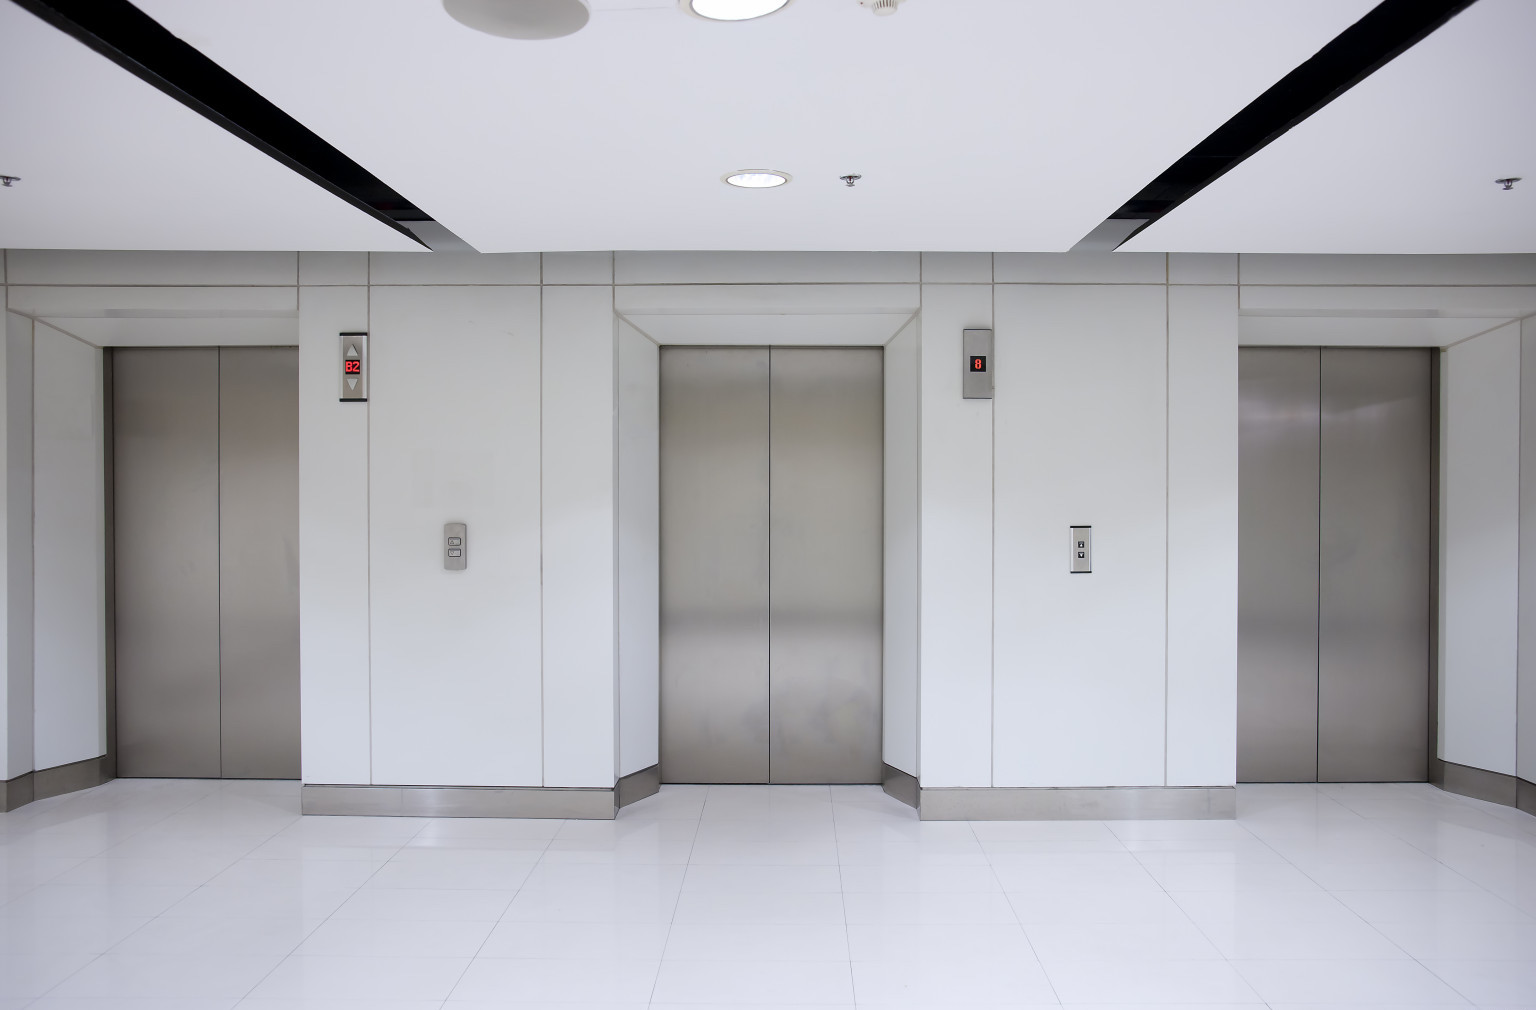
\includegraphics[width=1\textwidth]{src/elevators}}
\maketitle{}
\tableofcontents{}
\chapter{Motor}
\section{Stappenmotor}
Een stappenmotor(zie figuur~\ref{fig:stappenmotor}) werkt door stroom op bijvoorbeeld: fase 1,3,5 en 7 te plaatsen terwijl op fase 2,4,6 en 8 grond staat om de as 45 graden te laten draaien. Vervolgens zet je grond op waar stroom op heeft gezeten en vise versa.

\section{Direct current motor}
De DC motor(zie figuur~\ref{fig:dc_motor}) werkt door stroom te geven op het moment dat de motor de evenwichtssituatie nadert. Bij een stilstaande motor wordt er een puls gegeven om de motor een kwartslag te draaien waarna de ingebouwde magneten de motor verder draaien vanwege tegenwerkende polen. Als de motor weer richting de evenwichtssituatie gaat wordt er weer stroom gezet op de motor om hem weer uit deze positie te halen. Door deze herhaling blijft de motor draaien
\\
\begin{figure}[ht]
\begin{subfigure}{0.6\textwidth}
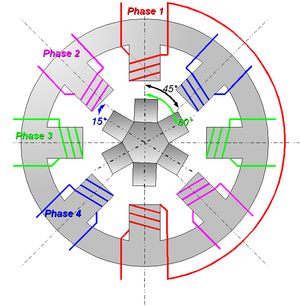
\includegraphics[height=5cm]{src/stepper_motor_schematic} 
\caption{Stappenmotor}
\label{fig:stappenmotor}
\end{subfigure}
\hfill
\begin{subfigure}{0.4\textwidth}
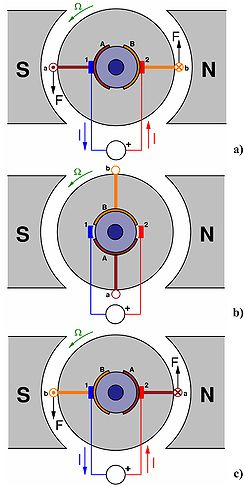
\includegraphics[height=5cm]{src/dc_motor_schematic}
\caption{DC motor}
\label{fig:dc_motor}
\end{subfigure}
\caption{Schematische weergave van de motoren}
\label{fig:motors}
\end{figure}

\section{Voor- en nadelen}
\begin{center}
\begin{tabular}{l|c|c} 
& Stappenmotor & DC motor \\
\hline
Nauwkeurig & \cmark & \xmark \\
\hline
Krachtig bij gelijk wattage & \cmark & \xmark \\
\hline
Simpel in gebruik & \xmark & \cmark \\
\hline
Prijs & \euro{12} - \euro{30} & \euro{5} - \euro{20}
\end{tabular}
\end{center}

\section{Advies}
Voor de motor adviseren wij een stappenmotor aan. Dit omdat in combinatie met de spoel(zie \ref{sec:spoel} voor meer informatie) een krachtige motor nodig is. Daarnaast kunnen wij de lift met een lage snelheid laten draaien zonder kracht te verliezen.
\chapter{Takel mechanisme}

\section{Contragewicht}
Een contragewicht(zie figuur~\ref{fig:contragewicht}) is een gewicht dat even zwaar is als de lift bij een gemiddelde lading. Als het gewicht van de lift wordt genomen en het gemiddelde gewicht van de lading, is dat het beste gewicht voor een contragewicht. Door een contragewicht te gebruiken hoeft de motor niet veel arbeid te leveren. Het gewicht van de lift is door het contragewicht opgeheven. 

\section{Spoel}\label{sec:spoel}
Een spoel(zie figuur~\ref{fig:spoel}) werkt door de lift aan een rol vast te binden en het touw omhoog te trekken samen met de lift om de lift te verplaatsen. het voordeel hiervan is dat dit een simpel systeem is. Deze methode kan al worden geïmplementeerd met alleen een motor, spoel en de lift aan een touw. Ook is de geleiding van alleen een lift makkelijker dan een lift met contragewicht. Je hoeft immers alleen rekening te houden met de lift zelf in plaats van de lift die zijn eigen plek heeft en het contragewicht.
\\
\begin{figure}[ht]
\begin{subfigure}{0.5\textwidth}
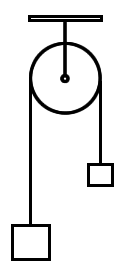
\includegraphics[height=5cm]{src/contragewicht} 
\caption{Contragewicht}
\label{fig:contragewicht}
\end{subfigure}
\hfill
\begin{subfigure}{0.5\textwidth}
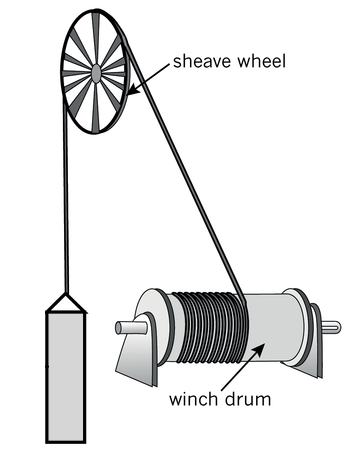
\includegraphics[height=5cm]{src/spoel}
\caption{Spoel}
\label{fig:spoel}
\end{subfigure}
\caption{Schematische weergave van takel mechanisme}
\label{fig:takel_mechanisme}
\end{figure}

\section{Voor- en nadelen}
\begin{center}
\begin{tabular}{l|c|c}
& Contragewicht & Spoel \\
\hline
Krachtige motor nodig & \xmark & \cmark \\
\hline
Complexe liftconstructie & \cmark & \xmark \\
\hline
Prijs & \euro{5} - \euro{10} & \euro{3} - \euro{6}
\end{tabular}
\end{center}

\section{Advies}
Hierbij adviseren wij een spoel. Dit omdat de spoel naar ons mening minder bouw \& ontwerp problemen met zich mee brengt dan een contragewicht.
\chapter{Materiaal}
\section{Hout}
Hout is een materiaal dat al heel lang wordt gebruikt met bouwen en dat is met een goede reden: het is sterk, redelijk flexiebel maar toch stevig en goedkoop. Het vraagt wel wat onderhoud om het voor een langere periode te kunnen gebruiken (lakken, schuren et cetera) maar voor een prototype is dit irrelevant. Een klein nadeel is dat met dikkere platen van bijvoorbeeld 6mm de plaat kan verbranden in de snijder. Dit vormt op zich geen gevaar als de machine goed ingesteld staat, maar voor zowel de uitstraling als de functionaliteit kan dit hinderend zijn.
\section{Plexiglas}
Plexiglas is een materiaal gemaakt uit een vorm van plastic die zeer geschikt is voor het bouwen van producten. Het is niet alleen onderhoudsvrij maar ook verkrijgbaar in veel verschillende kleuren en maten. Daarnaast is de grote reden dat wij dit materiaal willen gaan gebruiken dat het ook transparant uitgevoerd wordt. Hierdoor kan de bedrading en elektronische schakelingen makkelijk worden bekeken, begrepen en gerepliceerd worden voor eerstejaars. Het is dus niet belangrijk voor eerstejaars om dit materiaal te gaan gebruiken omdat deze niet de schakelingen hoeven te laten zien.

\section{Voor- en nadelen}
\begin{center}
\begin{tabular}{l|c|c}
& Hout & Plexiglas \\
\hline
Stevigheid & \cmark & \cmark \\
\hline
Doorzichtig & \xmark & \cmark \\
\hline
Prijs & \euro{3} & \euro{8}
\end{tabular}
\end{center}

\section{Advies}
Hierbij adviseren wij om de gehele lift van hout te maken. Plexiglas is niet meer vereist omdat onze elektronica zich voornamelijk aan de buiten kan zal bevinden en deze dus toch wel bekeken kan worden. Daarnaast is hout een stuk goedkoper.
\chapter{Communicatie}
Omdat dit project moet worden gemaakt door eerstejaars kijken wij alleen naar communicatieprotocollen die al ingebouwd zijn in de Arduino Uno/Mega.
 
\section{I\textsuperscript{2}C}
I\textsuperscript{2}C is een communicatieprotocol ontworpen om meerdere apparaten te laten communiceren door middel van het Master-Slave systeem. Dit communicatiesysteem is maar half-duplex, waardoor communicatie altijd maar een kant op kan. Dit zorgt ervoor dat de master altijd maar met 1 persoon tegelijk kan praten. Een nadeel is dat de slaves alleen mogen communiceren als de master hierom vraagt, waardoor de master continue alle slaves moet afgaan om veranderingen binnen te krijgen. Dit protocol is al ingebouwd in de Arduino.
 
\section{Serial}
Serial communicatie is een manier om 2 apparaten te laten communiceren. Dit systeem is full-duplex, maar kan maar met 1 apparaat praten. Dit is te overkomen door een Master-Slave te implementeren, waar de master Arduino met alle slaves kan communiceren, en de slaves alleen met de master kunnen communiceren. Het nadeel hiervan is dat er kans is op een data botsing als meerdere slaves tegelijk gaan praten.

\section{Voor- en nadelen}
\begin{center}
\begin{tabular}{l|c|c}
& I\textsuperscript{2}C & Serial \\
\hline
Communicatie richting & Half-duplex & Full-duplex \\
\hline
Meer dan 2 apparaten mogelijk & \cmark & \xmark/\cmark  \\
\hline
Onderling door linken & \cmark & \xmark \\
\hline
Geen data botsingen bij meer dan 2 apparaten & \cmark & \xmark \\
\end{tabular}
\end{center}

\section{Advies}
Ons advies voor communicatie is I\textsuperscript{2}C. Dit omdat I\textsuperscript{2}C gebouwd is voor communicatie tussen meerder apparaten. Daarnaast hebben wij maar twee pins op de master Arduino nodig om daarop alle Arduino's aan te sluiten, in tegenstelling tot Serieel waar voor elke slave Arduino twee pins nodig zijn.
\chapter{Initialisatie liftsysteem}
Omdat het liftsysteem modulair moet zijn, is het belangrijk dat er een manier wordt gevonden om te registreren welke verdieping waar zit en waar de lift zich bevindt.
 
\section{Handmatig instellen}
Het vooraf instellen van de liften als deze in een bepaalde configuratie zijn geplaatst is een goede manier om betrouwbaar de lift in te stellen. Omdat bij een modulair systeem de lift delen verwisseld moeten kunnen worden, is het instellen van de verdiepingen met de hand redelijk snel en eenvoudig te implementeren en wat langzamer om in te stellen als de lift delen zijn verplaatst. De lift delen doen hiermee niet automatisch registreren op welke verdieping ze zijn.

\section{Vooraf geprogrammeerd}
Het vooraf programmeren van een lift deel houdt in dat er in de code van dat specifieke lift deel al een verdieping is ingesteld. Dit houd in dat de lift delen in een vaste volgorde moeten worden geassembleerd maar betekent dat de lift minder tijd nodig heeft om ingesteld te worden.
 
\section{Automatisch instellen}
Met automatisch instellen wordt de lift bij opstarten op de begane grond gezet en zal er gekeken worden welk device de lift registreert. Vervolgens gaat de lift omhoog en blijft deze registreren op welke verdieping de lift wordt gezien. Als de lift boven is beëindigd deze routine en weet de lift waar welke verdieping is en kan de lift geregeld worden


\section{Voor- en nadelen}
\begin{center}
\begin{tabular}{l|c|c|c}
& Handmatig instellen & Vooraf geprogrammeren & Automatisch \\
\hline
Programmeerbaarheid & makkelijk & zeer makkelijk & zeer moeilijk \\
\hline
Insteltijd & redelijk snel & zeer snel & snel \\
\hline
Modulair & \cmark & \xmark & \cmark \\
\end{tabular}
\end{center}

\section{Advies}
Ons advies is om voor handmatig instellen te gaan omdat  dit makkelijk te programmeren is en voor voldoende flexibiliteit zorgt.
\chapter{Lift detectie}

\section{IR: infrarood}
De infrarood sensor kan zien of het licht dat de sensor uitstuurt terugkomt op de sensor. Door bijvoorbeeld een reflector te plaatsen op de lift kan een verdieping zien of het licht terugkomt via de reflector en dus of de lift aanwezig is op dat moment of niet. Dit systeem is makkelijk te implementeren en in te programmeren.

\section{Limit switch}
Een limit switch is een knop die wordt ingedrukt als de lift er langs gaat. De lift drukt de switch in op het moment dat de lift de hoogte van de switch bereikt. Deze methode is zeer betrouwbaar omdat als een switch eenmaal is geïnstalleerd en vast zit, het weinig defecten kan vertonen. Het installeren van deze switch is wat moeilijker omdat de liftkooi goed vast op geleiders moet zitten zodat de switch daadwerkelijk ingedrukt wordt als de lift langskomt en dat de lift niet vast komt te zitten omdat de switch de lift uit de geleiders drukt.

\section{Magnetische reedcontacten}
Magnetische reedcontacten werken door een stuk metaal op de lift te plaatsen die kan worden gedetecteerd door een sensor op de verdieping. Het moment dat de lift langs komt zal de magneetsensor het stukje metaal zien en kan de lift gedetecteerd worden. Een magnetisch reedcontact kan een stukje metaal detecteren zelfs als de lift niet volledig stabiel door de schacht gaat.

\section{Voor- en nadelen}
\begin{center}
\begin{tabular}{l|c|c|c}
& IR & Limit switch & Magnetisch \\
\hline
Betrouwbaar & \cmark & \cmark & \cmark \\
\hline
Makkelijk implementeerbaar & \cmark & \xmark & \cmark \\
\hline
Precisie detectie & 5 mm & 1 mm & 20 mm \\
\hline
Prijs & \euro{7,50} & \euro{10} & \euro{7,50} \\

\end{tabular}
\end{center}

\section{Advies}
Voor de lift detectie adviseren wij infrarood aan, omdat infrarood zowel betrouwbaar is als makkelijk te implementeren.
\end{document}
